\documentclass[tikz,border=10pt]{standalone}
\usepackage{tikz}
\usetikzlibrary{arrows.meta, positioning, shapes.geometric, fit, backgrounds, shadows}

\definecolor{clrBrowser}{HTML}{1A3A5C}
\definecolor{clrAPI}{HTML}{2D5016}
\definecolor{clrHeuristic}{HTML}{4A2070}
\definecolor{clrRunner}{HTML}{6B3010}
\definecolor{clrAlgo}{HTML}{1A4A4A}
\definecolor{clrDijkstra}{HTML}{5C1A1A}
\definecolor{clrResult}{HTML}{2D4A1A}
\definecolor{clrBrowser2}{HTML}{1A3A5C}
\definecolor{clrArrow}{HTML}{C9A84C}
\definecolor{clrBg}{HTML}{0F1923}
\definecolor{clrLabel}{HTML}{8AABCC}

\begin{document}
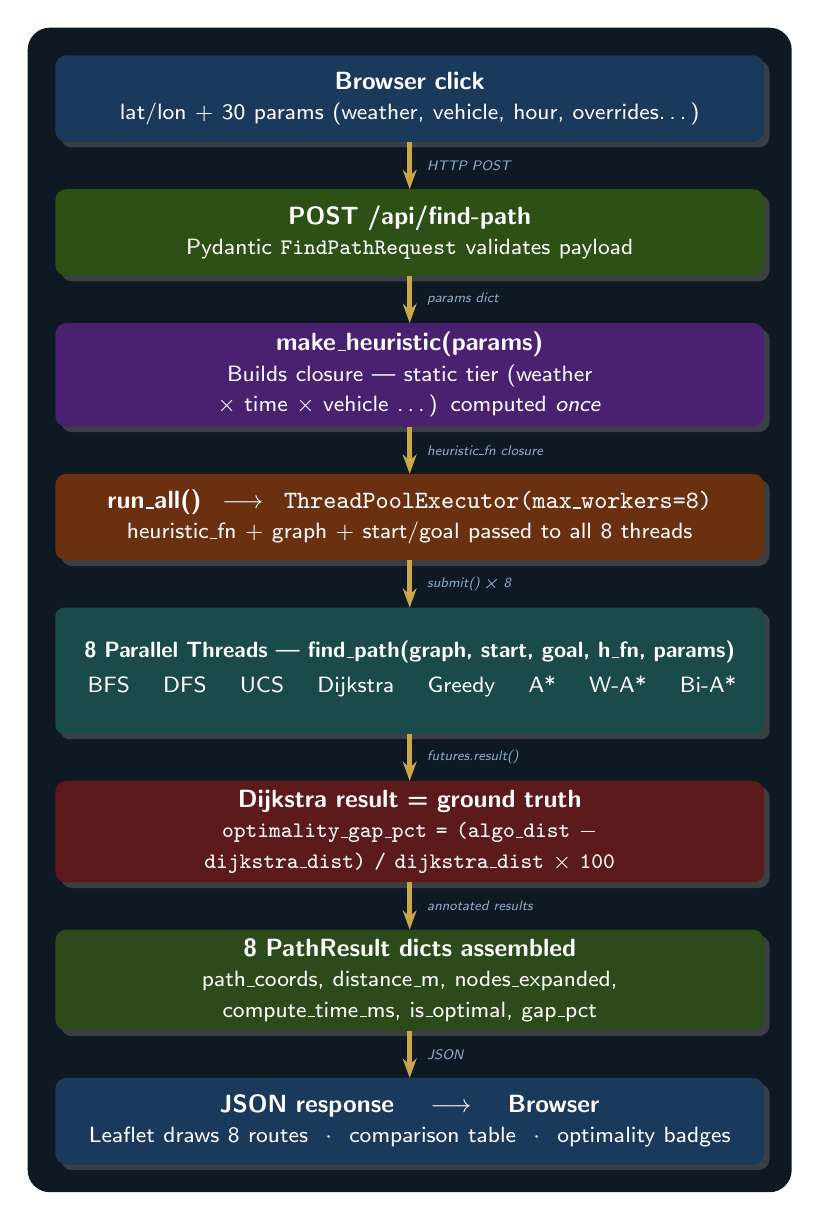
\begin{tikzpicture}[
  node distance = 0mm,
  box/.style = {
    rectangle,
    rounded corners=4pt,
    minimum width=9cm,
    minimum height=1.1cm,
    text width=8.6cm,
    align=center,
    font=\sffamily\small,
    text=white,
    drop shadow={shadow xshift=2pt, shadow yshift=-2pt, fill=black!60}
  },
  arrow/.style = {
    -{Stealth[length=7pt, width=5pt]},
    line width=1.6pt,
    color=clrArrow
  },
  label/.style = {
    font=\sffamily\tiny\itshape,
    text=clrLabel,
    align=left
  },
  every node/.style={outer sep=0pt}
]

% ── nodes ────────────────────────────────────────────────────────────────────

\node[box, fill=clrBrowser] (browser)
  {\textbf{Browser click}\\
   \footnotesize lat/lon + 30 params (weather, vehicle, hour, overrides\ldots)};

\node[box, fill=clrAPI, below=6mm of browser] (api)
  {\textbf{POST /api/find-path}\\
   \footnotesize Pydantic \texttt{FindPathRequest} validates payload};

\node[box, fill=clrHeuristic, below=6mm of api] (heuristic)
  {\textbf{make\_heuristic(params)}\\
   \footnotesize Builds closure — static tier (weather $\times$ time $\times$ vehicle \ldots) computed \textit{once}};

\node[box, fill=clrRunner, below=6mm of heuristic] (runner)
  {\textbf{run\_all()} $\;\longrightarrow\;$ \texttt{ThreadPoolExecutor(max\_workers=8)}\\
   \footnotesize heuristic\_fn + graph + start/goal passed to all 8 threads};

% ── algo row ─────────────────────────────────────────────────────────────────
\node[
  rectangle, rounded corners=3pt,
  fill=clrAlgo,
  minimum width=9cm, minimum height=1.6cm,
  text width=8.6cm, align=center,
  font=\sffamily\footnotesize, text=white,
  drop shadow={shadow xshift=2pt, shadow yshift=-2pt, fill=black!60},
  below=6mm of runner
] (algos) {
  \textbf{8 Parallel Threads — find\_path(graph, start, goal, h\_fn, params)}\\[3pt]
  \footnotesize
  \begin{tabular}{cccccccc}
  BFS & DFS & UCS & Dijkstra & Greedy & A* & W-A* & Bi-A*
  \end{tabular}
};

\node[box, fill=clrDijkstra, below=6mm of algos] (dijkstra)
  {\textbf{Dijkstra result = ground truth}\\
   \footnotesize \texttt{optimality\_gap\_pct = (algo\_dist $-$ dijkstra\_dist) / dijkstra\_dist $\times$ 100}};

\node[box, fill=clrResult, below=6mm of dijkstra] (results)
  {\textbf{8 PathResult dicts assembled}\\
   \footnotesize path\_coords, distance\_m, nodes\_expanded, compute\_time\_ms, is\_optimal, gap\_pct};

\node[box, fill=clrBrowser2, below=6mm of results] (frontend)
  {\textbf{JSON response $\;\longrightarrow\;$ Browser}\\
   \footnotesize Leaflet draws 8 routes $\;\cdot\;$ comparison table $\;\cdot\;$ optimality badges};

% ── arrows ───────────────────────────────────────────────────────────────────
\draw[arrow] (browser)   -- node[label, right=3pt] {HTTP POST} (api);
\draw[arrow] (api)       -- node[label, right=3pt] {params dict} (heuristic);
\draw[arrow] (heuristic) -- node[label, right=3pt] {heuristic\_fn closure} (runner);
\draw[arrow] (runner)    -- node[label, right=3pt] {submit() × 8} (algos);
\draw[arrow] (algos)     -- node[label, right=3pt] {futures.result()} (dijkstra);
\draw[arrow] (dijkstra)  -- node[label, right=3pt] {annotated results} (results);
\draw[arrow] (results)   -- node[label, right=3pt] {JSON} (frontend);

% ── background panel ─────────────────────────────────────────────────────────
\begin{pgfonlayer}{background}
  \node[
    fill=clrBg,
    rounded corners=8pt,
    inner sep=10pt,
    fit=(browser)(api)(heuristic)(runner)(algos)(dijkstra)(results)(frontend)
  ] {};
\end{pgfonlayer}

\end{tikzpicture}
\end{document}
